\documentclass{article}
\usepackage[utf8]{inputenc}
\usepackage{graphicx}
\usepackage[fleqn]{mathtools} 
\usepackage{textcomp}
\usepackage{titling}
\usepackage{subfig}
\usepackage[parfill]{parskip}
\usepackage{xcolor}
\definecolor{LightGray}{gray}{0.9}
\usepackage{titlesec}
\setcounter{secnumdepth}{4}
\usepackage[a4paper,left=1cm,right=1cm,top=1cm,bottom=1.5cm,]{geometry}
\usepackage{eqparbox}
\usepackage{enumitem}
\usepackage{relsize}
\usepackage{dsfont}

\title{\vspace{-2cm} CS231N Assignment 1 - SVM}
\date{\vspace{-5ex}}

\begin{document}
\maketitle

\section{Soft SVM - Introduction}
In contrast with the hard SVM that we learned in CS3244.

\subsection{What's wrong with the Hard SVM?}
In hard SVM, the optimization problem enforces that all points in training must be classified correctly.
However in practical cases, noise prevents/limits the existence of a hyperplane that \textbf{perfectly} seperates the data, in which case the hard SVM optimization returns no/poor solutions.

Alternatively, a single outlier determines the boundary in the hard SVM, making it overly sensitive to noise in data
\begin{figure}[htp]
    \centering
    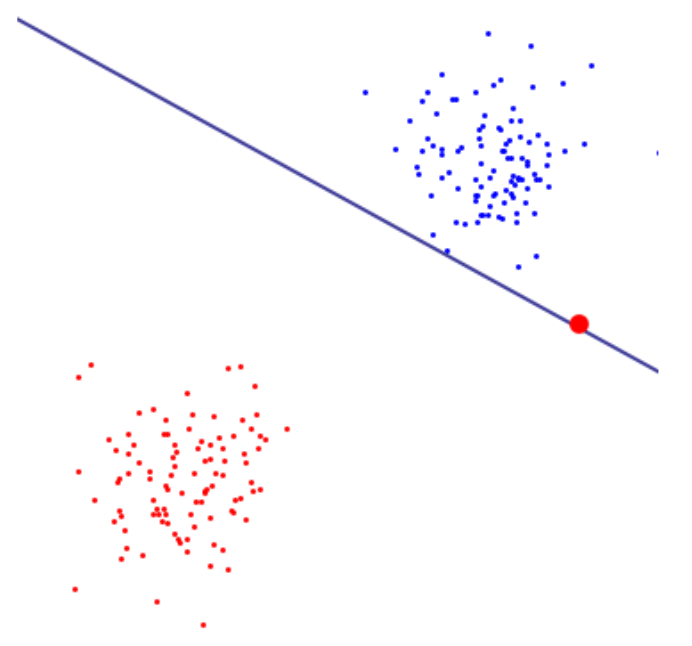
\includegraphics[width=4cm, scale=1]{images/hardSVM.PNG}
    \caption{Single red outlier determines boundary - hallmark of overfitting}
\end{figure}

\subsection{Developing a Soft SVM}
Therefore, we modify the hard SVM to allow for some training points to be missclassified.

To do this, we introduce \textit{slack variables} $\xi_{n} \ge 0$, one slack variable for each training data point.

\subsubsection{Modifiying the classification constraint}
\begin{itemize}
    \item Classification constraints are now $t_{n}y_{n}(x_{n}) \ge 1 - \xi_{n}$, in which slack variables constrained to satisfy $\xi_{n} \ge 0$
        \begin{itemize}
            \item Recall that $y_{n}(x_{n}) = w^{T}x_{n}+b$
        \end{itemize}
    \item Data points for which $\xi_{n} = 0$ are correctly classified (either on the margin or on the correct side of the margin)
    \item Points for which $0 < \xi_{n} \le 1$ lie inside the margin, but on the correct side of the decision boundary
    \item Points for which $\xi_{n} > 1$ lie on the wrong side of the decision boundary and are \textbf{misclassified}
    \item One choice of $\xi_{n}$ would be the \textit{hinge loss}
        \begin{itemize}
            \item Hinge loss = $max\{0, 1-y_{n}(w^{T}x_{n}+b)\}$
        \end{itemize}
\end{itemize}

\subsubsection{Our new optimization goal now}
We want to maximize the margin while \textbf{penalizing points that lie on wrong side of the decision boundary}.

Therefore, \textbf{minimize} $\Bigl\{C\sum\limits_{n=1}^{N}\xi_{n} + \frac{||w||^{2}}{2}\Bigr\}$ subject to constraints $t_{n}y_{n}(x_{n}) \ge 1 - \xi_{n}$; $\xi_{n} \ge 0$
\begin{itemize}
    \item \textbf{Regularization} parameter $C$ controls the trade-off between maximizing the margin and minimizing the loss
\end{itemize}

Similar to the hard SVM case, we can solve this by forming converting from primal lagrangian to dual lagragian (See PRML).
We will observe that the dual lagrangian of the soft SVM only differs by an upper bound applied to the Lagrange multipliers.

\newpage
\section{Multiclass SVM Loss - CS231N}
CS231N terms this 'SVM' loss, although this is not really accurate (we are just looking at the hinge loss term). We will use these two terms interchangeably.

\subsection{Recap on loss functions}
\begin{itemize}
    \item Suppose we have dataset of examples $\Bigl\{(x_{i}, y_{i})\Bigr\}^{N}_{i=1}$; $x_{i}$ is image, $y_{i}$ is label
    \item Suppose we have some linear classifier $f(x_{i},W)$; $W$ is some weight matrix
    \item Loss for a \textbf{single} example defined as $L_{i} = (f(x_{i},W),y_{i})$
    \item Loss for \textbf{entire dataset} defined as average of per-example loss; $L = \frac{1}{N}\sum_{i}L_{i}(f(x_{i},W),y_{i})$
\end{itemize}

\subsection{Visualizing linear classifiers}
\subsubsection{Algebraic viewpoint}
\begin{figure}[htp]
    \centering
    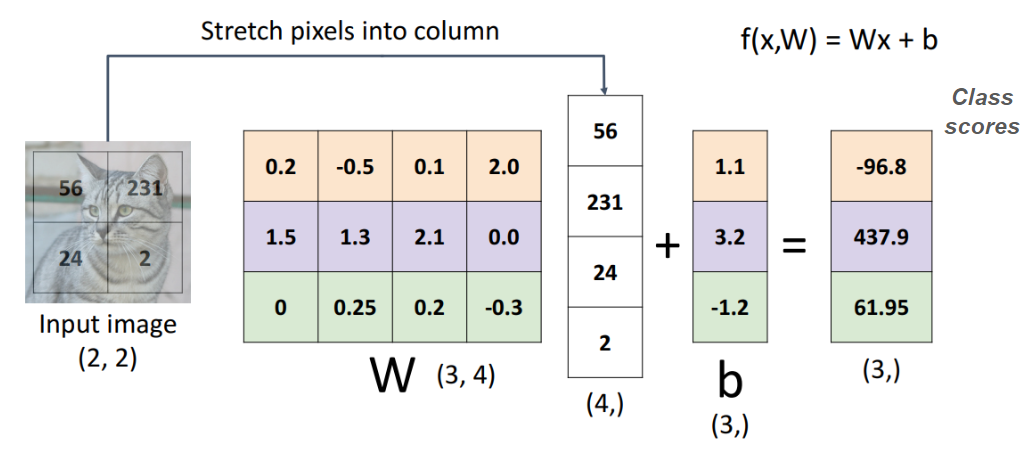
\includegraphics[width=12cm, scale=1]{images/algebraicViewpoint.PNG}
    \caption{Weight matrix has it's own preference for each class, weighting the input image appropriately}
\end{figure}

\subsubsection{Template viewpoint}
\begin{figure}[htp]
    \centering
    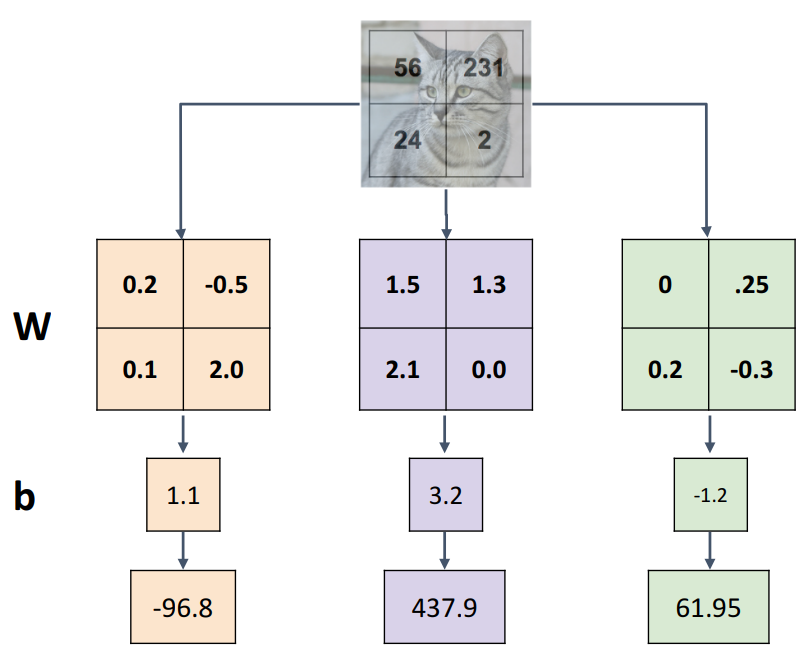
\includegraphics[width=10cm, scale=1]{images/templateViewpoint.PNG}
    \captionsetup{justification=centering}
    \caption{Transform weight matrix into same dimension as input image, then do dot product\\
                Recall that dot product is a measure of similarity}
\end{figure}

\newpage
\subsubsection{Visual viewpoint}
\begin{figure}[htp]
    \centering
    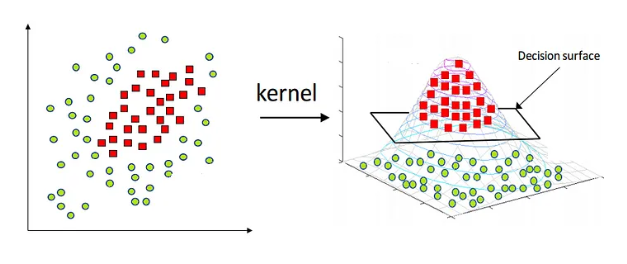
\includegraphics[width=12cm, scale=1]{images/visualViewpoint.png}
    \caption{Hyperplane seperating points (after kernel transformation)}
\end{figure}

\subsection{Multiclass SVM Loss}
\begin{itemize}
    \item Suppose for some $i_{th}$ training example, we are given the pixels of image $x_{i}$ and the label $y_{i}$ that specifies the index of the correct class
    \item We have a linear classifier $f(x_{i},W)$ that outputs a \textbf{vector} $\boldsymbol{v}$ of \textit{class scores} (closeness of $x_{i}$ to all labels $y$)
        \begin{itemize}
            \item eg. $j_{th}$ class score = $v_{j} = f(x_{i},W)_{j}$
        \end{itemize}
    \item Define the Multiclass SVM loss for the $i_{th}$ example as $L_{i} = \mathlarger{\sum\limits}_{j \neq y_{i}}max(0, s_{j}-s_{y_{i}} + \Delta)$; $y_{i}$ is the 'true' class
        \begin{itemize}
            \item Since we are working with linear classifiers (ie. $f(x_{i},W) = Wx_{i}$), we can rewrite the loss function as\\
                    $L_{i} = \mathlarger{\sum\limits}_{j \neq y_{i}}max(0, W_{j}^{T}x_{i} - W_{y_{i}}^{T}x_{i} + \Delta)$
                        \begin{itemize}
                            \item $W_{j}$ is $j_{th}$ row of weight matrix W
                            \item $W_{y_{i}}$ is the row of weight matrix W corresponding to the \textbf{correct} class label $y_{i}$
                            \item Assuming that vectors $x_{i}$ are \textbf{row} vectors, we transpose the weight matrices into \textbf{column} vectors to make mmult dimensions work
                        \end{itemize}
            \item Given some image $x_{i}$, it's correct class score $s_{y_{i}}$ must be larger than \textbf{all} incorrect class scores by at least $\Delta$. Otherwise loss will be incurred.
        \end{itemize}
\end{itemize}

\begin{minipage}[t]{0.5\textwidth}
    \centering
    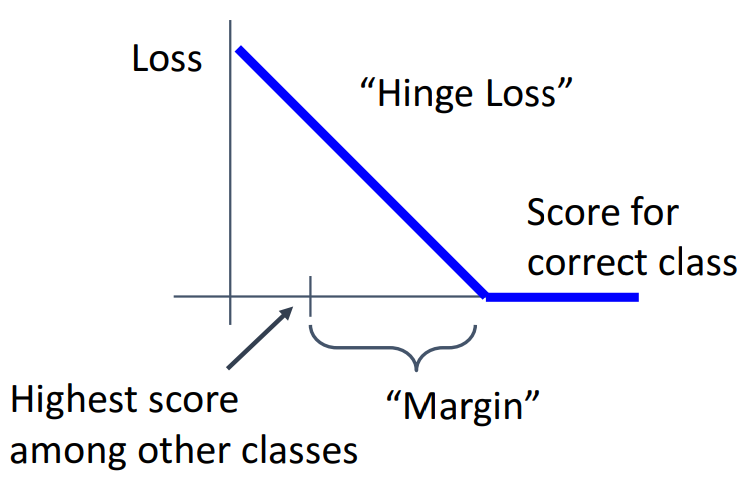
\includegraphics[width=8cm, scale=1]{images/hingeLoss.PNG}
    \captionof{figure}{Hinge Loss}
\end{minipage}%
\begin{minipage}[t]{0.5\textwidth}
    \centering
    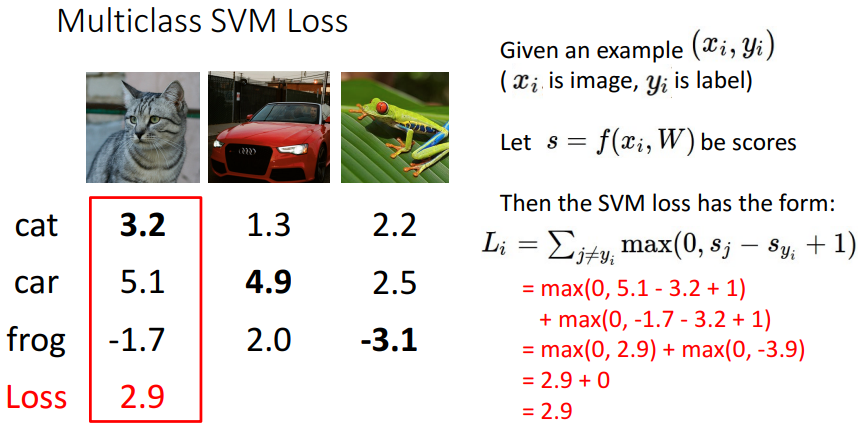
\includegraphics[width=8cm, scale=1]{images/hingeExample.PNG}
    \captionsetup{justification=centering}
    \captionof{figure}{Example calculation}
\end{minipage}%

\subsection{Gradient of Hinge Loss - Single datapoint}
\begin{equation}
    \text{We know that the multiclass SVM loss is }
    L_{i} = \mathlarger{\sum\limits}_{j \neq y_{i}}max(0, W_{j}^{T}x_{i} - W_{y_{i}}^{T}x_{i} + \Delta)
\end{equation}

\begin{subequations}
    \renewcommand{\theequation}{\theparentequation.\arabic{equation}}
    \begin{equation}
        \text{We can split this up as a piecewise function } L_{i} = 
        \begin{cases} 
            \mathlarger{\sum\limits}_{j \neq y_{i}}(W_{j}^{T}x_{i} - W_{y_{i}}^{T}x_{i} + \Delta) & \text{if } W_{y_{i}}^{T}x_{i} < W_{j}^{T}x_{i} + \Delta  \\[2em]
            0 & \text{otherwise}
        \end{cases}
    \end{equation}
    \begin{equation}
        \begin{split}
            &\text{Intuitively, this is saying that we incur non-zero error whenever the correct class score } W_{y_{i}}^{T}x_{i} = s_{y_{i}} \\
            &\text{is not larger than all other incorrect class scores by } \Delta
        \end{split}
    \end{equation}
\end{subequations}

\begin{subequations}
    \renewcommand{\theequation}{\theparentequation.\arabic{equation}}
    \begin{equation}
        \begin{split}
            &\text{We are doing a scalar-by-matrix derivative, arranged in denominator layout}\\[1em]
            &\mathlarger{\mathlarger{\nabla_{\boldsymbol{W}}L_{i} = 
                                    \frac{\partial L_{i}}{\partial \boldsymbol{W}}} =
                                    \begin{bmatrix}
                                        \frac{\partial L_{i}}{W_{11}} & \frac{\partial L_{i}}{W_{12}} & \dots &  \frac{\partial L_{i}}{W_{1p}}\\[0.5em]
                                        \frac{\partial L_{i}}{W_{21}} & \frac{\partial L_{i}}{W_{22}} & \dots &  \frac{\partial L_{i}}{W_{2p}}\\[0.5em]
                                        \vdots & \vdots & & \vdots \\
                                        \frac{\partial L_{i}}{W_{j1}} & \frac{\partial L_{i}}{W_{j2}} & \dots &  \frac{\partial L_{i}}{W_{jp}}\\[0.5em]
                                        \vdots & \vdots & & \vdots \\
                                        \frac{\partial L_{i}}{W_{n1}} & \frac{\partial L_{i}}{W_{n2}} & \dots &  \frac{\partial L_{i}}{W_{np}}\\[0.5em]
                                    \end{bmatrix}}\\
            &\text{Let us proceed to derive the hinge loss' gradient } \textbf{for the case where error is incurred}
        \end{split}
    \end{equation}\vspace{1cm}
    \begin{equation}
        \mathlarger{\mathlarger{\mathlarger{\nabla_{w_{y_{i}}}}}L_{i} = 
                                            -\sum\limits_{j\neq y_{i}} x_{i}}
    \end{equation}
    \begin{equation}\tag{3.2.1}
        \text{This is saying that we scale } x_{i} \text{ by the number of classes that didn't meet the margin } \Delta
    \end{equation}
    \begin{equation}\tag{3.2.2}
        \begin{split}
            & \text{Note that this is the gradient only with respect to the row of } \boldsymbol{W} \text{ that corresponds to the correct class}\\
            & \text{Recall that } W_{y_{i}} \text{ corresponds to row of weight matrix } \boldsymbol{W}\\
            & \text{ie. We are doing a scalar-by-vector derivative that provides us with a row of } \frac{\partial L_{i}}{\boldsymbol{W}} \text{, as seen below}\\[0.5em]
            &\mathlarger{\mathlarger{\frac{\partial L_{i}}{\partial \boldsymbol{W}_{y_{i}}}} =
                                    \begin{bmatrix}
                                        \frac{\partial L_{i}}{W_{y_{i}1}} & \frac{\partial L_{i}}{W_{y_{i}2}} & \dots & \frac{\partial L_{i}}{W_{y_{i}p}}\\[0.5em]
                                    \end{bmatrix}}\\
        \end{split}
    \end{equation}\vspace{1cm}
    \begin{equation}
        \begin{split}
        & \text{Hence for the other rows of } \nabla_{\boldsymbol{W}}L_{i} \text{, we have that }
            \mathlarger{\mathlarger{\mathlarger{\nabla_{w_{j}}}}L_{i} = x_{i}}
        \end{split}
    \end{equation}
\end{subequations}

\subsection{Regularization}
\subsubsection{Intuition}
Set of $\boldsymbol{W}$ that correctly classifies (ie. $L_{i} = 0$ for all i) is \textbf{not unique}.\\
Intuitively speaking this is true. If some $\boldsymbol{W}$ satisfies that $L_{i} = 0 \ \forall i$, then $\lambda \boldsymbol{W}; \lambda > 1$ also satifies that.

\begin{figure}[htp]
    \centering
    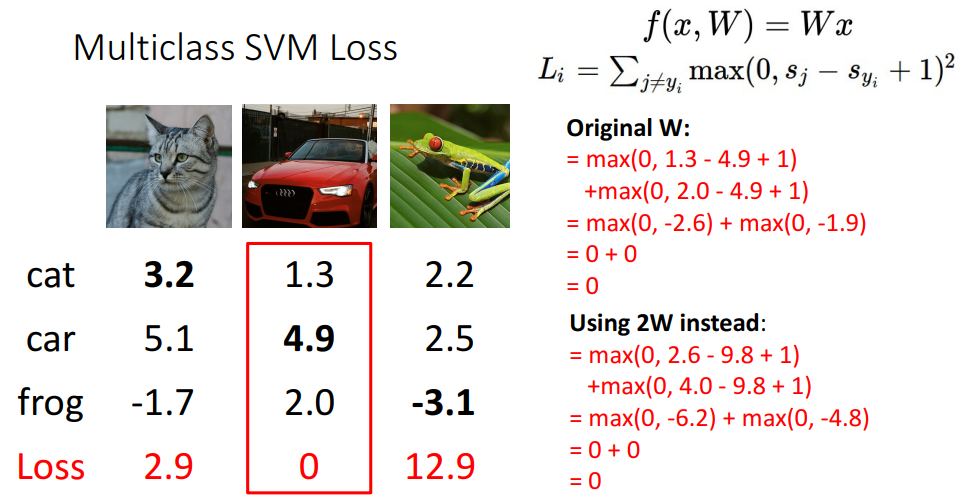
\includegraphics[width=10cm, scale=1]{images/nonUniqueWeights.PNG}
    \caption{Non-uniqueness of weights}
\end{figure}

\subsection{Regularization term}
We want to encode some preference for a certain set of weights $\boldsymbol{W}$ over others to remove this ambiguity.\\
We can do so by extending the loss function with a regularization penalty $R(W)$.\\
Common $R(W)$ is the \textit{Squared L2 norm}, which discourages large weights through a quadratic penalty.

\begin{figure}[htp]
    \centering
    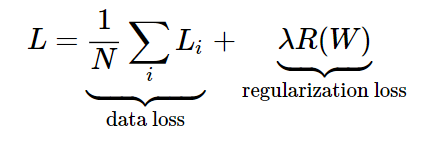
\includegraphics[width=10cm, scale=1]{images/regularizationFormula.PNG}
    \captionsetup{justification=centering}
    \caption{Notice that $R(W)$ is function of weights only, not data\\
                Intuitively speaking, smaller weights are preferred since they generalize better (no input dimension can have very large influence on scores all by itself)}
\end{figure}

\subsection{Gradient of Hinge Loss - All datapoints}
Let's attempt to calculate gradient of hinge loss for \textbf{all} datapoints in a non-naive way
\setcounter{equation}{0}

\begin{subequations}
    \renewcommand{\theequation}{\theparentequation.\arabic{equation}}
    \begin{equation}
        \text{Define } \mathlarger{margin_{ij} = W_{j}^{T}x_{i} - W_{y_{i}}^{T}x_{i} + \Delta}
    \end{equation}
    \begin{equation}
        \text{Rewrite } \mathlarger{L_{i} = \sum\limits_{j \neq y_{i}}max(0, W_{j}^{T}x_{i} - W_{y_{i}}^{T}x_{i} + \Delta) = \sum\limits_{j \neq y_{i}}max(0, margin_{ij})}
    \end{equation}\vspace{0.25cm}
    \begin{equation}
        \text{Let's rederive the partial derivatives, but not breaking it up into piecewise function as we did previously}
    \end{equation}
    \begin{equation}\tag{1.3.1}
        \begin{split}
            \mathlarger{\nabla W_{y_{i}} L_{i}} & = \mathlarger{\nabla W_{y_{i}}\Bigl\{\sum\limits_{j \neq y_{i}}max(0, W_{j}^{T}x_{i} - W_{y_{i}}^{T}x_{i} + \Delta)\Bigr\}}\\
                                                & = \mathlarger{-\sum\limits_{j \neq y_{i}}\mathds{1}_{>0}(W_{j}^{T}x_{i} - W_{y_{i}}^{T}x_{i} + \Delta)x_{i}}\\
                                                & = \mathlarger{-\sum\limits_{j \neq y_{i}}\mathds{1}_{>0}(margin_{ij})x_{i}}
        \end{split}
    \end{equation}
    \begin{equation}\tag{1.3.2}
        \begin{split}
            \mathlarger{\nabla W_{j} L_{i}} & = \mathlarger{\nabla W_{j}\Bigl\{\sum\limits_{j \neq y_{i}}max(0, W_{j}^{T}x_{i} - W_{y_{i}}^{T}x_{i} + \Delta)\Bigr\}}\\
                                            & = \mathlarger{\mathds{1}_{>0}(W_{j}^{T}x_{i} - W_{y_{i}}^{T}x_{i} + \Delta)x_{i}}\\
                                            & = \mathlarger{\mathds{1}_{>0}(margin_{ij})x_{i}}\\
        \end{split}
    \end{equation}\vspace{0.25cm}
    \begin{equation}
        \text{Let's derive equations of the partial derivatives, for all datapoints now}
    \end{equation}
    \begin{equation}\tag{1.4.1}
        \begin{split}
            \mathlarger{\nabla W_{y} L} & = \mathlarger{\nabla W_{y}\Bigl\{\frac{1}{N}\sum\limits_{i}^{N}L_{i}\Bigr\}} \text{; $\boldsymbol{W}_{y}$ is rows of $\boldsymbol{W}$, y represents all correct class labels}\\
                                        & = \mathlarger{\frac{1}{N} \sum\limits_{i}^{N} \Bigl\{ \nabla W_{y_{i}}L_{i} \Bigr\}}\\
                                        & = \mathlarger{\frac{1}{N} \sum\limits_{i}^{N} \Bigl\{ \sum\limits_{j \neq y_{i}}-\mathds{1}_{>0}(margin_{ij})x_{i}  \Bigr\}}
        \end{split}
    \end{equation}
    \begin{equation}\tag{1.4.2}
        \begin{split}
            \mathlarger{\nabla W_{j} L} & = \mathlarger{\nabla W_{j}\Bigl\{\frac{1}{N}\sum\limits_{i}^{N}L_{i}\Bigr\}} \text{; j is our loop iterator}\\
                                        & = \mathlarger{\frac{1}{N} \sum\limits_{i}^{N} \Bigl\{ \nabla W_{j}L_{i} \Bigr\}}\\
                                        & = \mathlarger{\frac{1}{N} \sum\limits_{i}^{N} \Bigl\{ \mathds{1}_{>0}(margin_{ij})x_{i}\Bigr\}}
        \end{split}
    \end{equation}
\end{subequations}

\newpage
\subsubsection{Vectorized Dot Product approach}
Let's build some intuition using a toy example first. Note that matrix values are not accurate, they are just for illustration

\begin{figure}[htp]
    \centering
    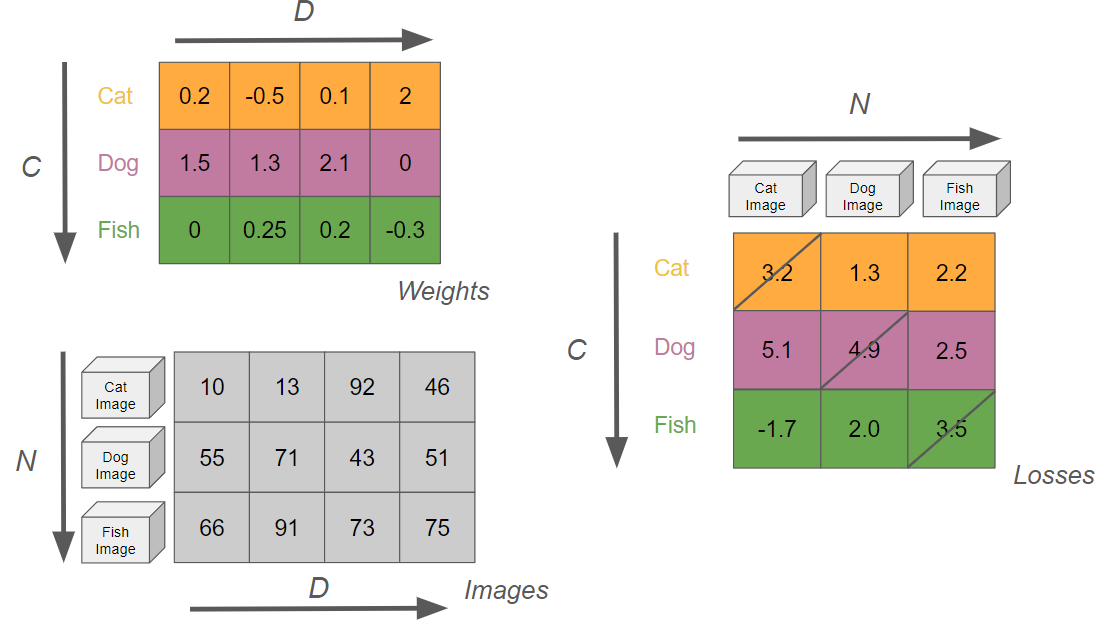
\includegraphics[width=12cm, scale=1]{images/overView.PNG}
    \captionsetup{justification=centering}
    \caption{C (number of classes) = 3\\
             D (data dimension) = 4\\
             N (number of samples) = 3}
\end{figure}

\begin{itemize}
    \item Let us consider how $\frac{\partial L_{i}}{\partial \boldsymbol{W}}$ is calculated, taking cat image as an example
        \begin{itemize}
            \item $\mathlarger{\mathlarger{\mathlarger{\nabla_{W_{y_{i}}}L_{i} = -\sum\limits_{j \neq y_{i}}\mathds{1}_{>0}(margin_{ij})x_{i}}}}$
            \item $\mathlarger{\mathlarger{\mathlarger{\nabla_{w_{j}}L_{i} = \mathds{1}_{>0}(margin_{ij})x_{i}}}}$
        \end{itemize}
\end{itemize}

\begin{minipage}[t]{0.5\textwidth}
    \centering
    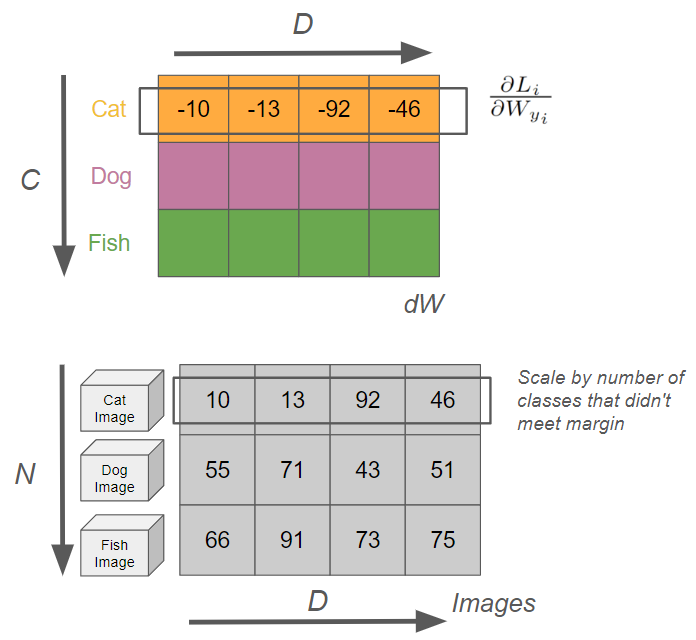
\includegraphics[width=5cm, scale=1]{images/toy1.PNG}
    \captionsetup{justification=centering}
    \captionof{figure}{Dog class margin did not meet $\Delta$ constraint}
\end{minipage}%
\begin{minipage}[t]{0.5\textwidth}
    \centering
    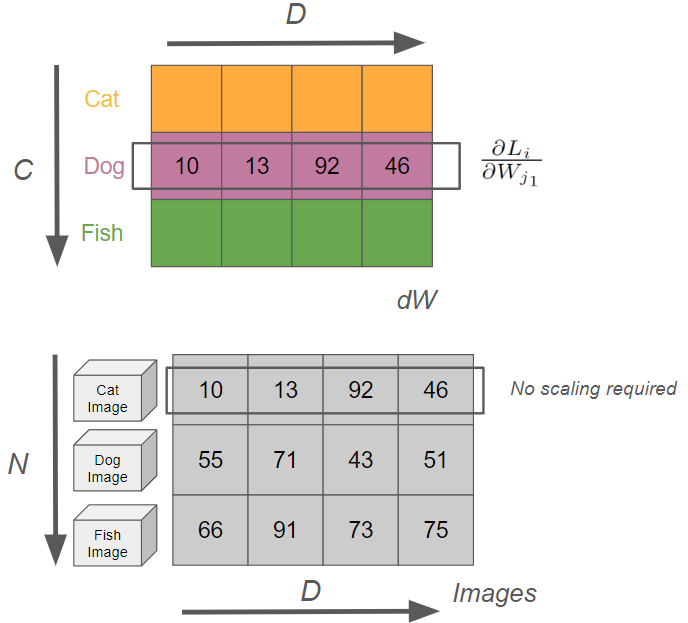
\includegraphics[width=5cm, scale=1]{images/toy2.PNG}
    \captionsetup{justification=centering}
    \captionof{figure}{No scaling required (as per derivation calculation)}
\end{minipage}%

\begin{figure}[htp]
    \centering
    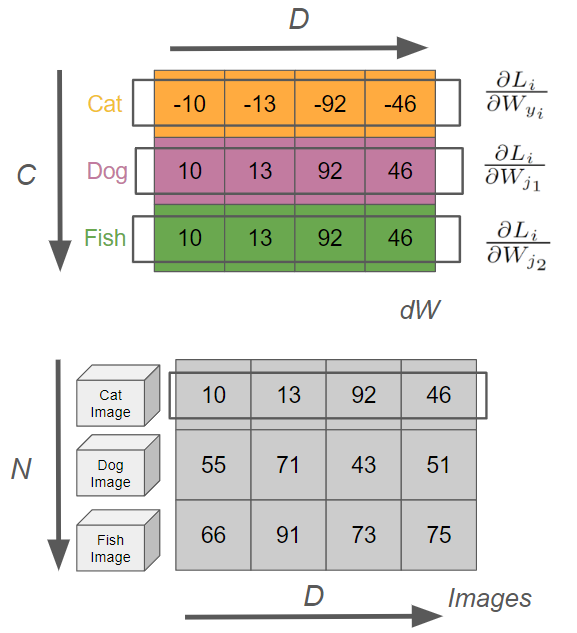
\includegraphics[width=5cm, scale=1]{images/toy3.PNG}
    \captionsetup{justification=centering}
    \caption{Final dW matrix for $L_{i}$ corresponding to cat image}
\end{figure}

\newpage
\begin{itemize}
    \item Note the key discovery here $\dots$
\end{itemize}

\begin{minipage}[t]{0.5\textwidth}
    \centering
    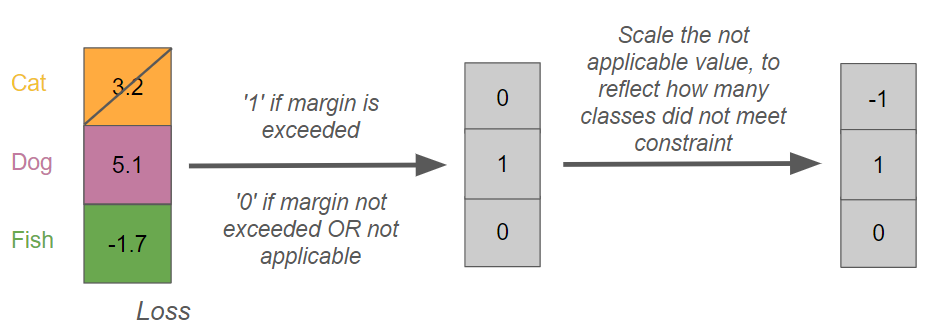
\includegraphics[width=8cm, scale=1]{images/keyPoint1.PNG}
    \captionsetup{justification=centering}
    \captionof{figure}{Convert \textit{Loss} to a 'flag' matrix}
\end{minipage}%
\begin{minipage}[t]{0.5\textwidth}
    \centering
    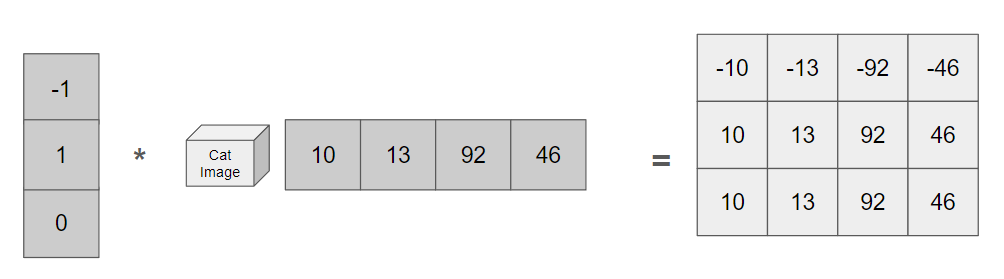
\includegraphics[width=10cm, scale=1]{images/keyPoint2.PNG}
    \captionsetup{justification=centering}  
    \captionof{figure}{Strang's Row-Matrix multiplication idea}
\end{minipage}%




\end{document}